
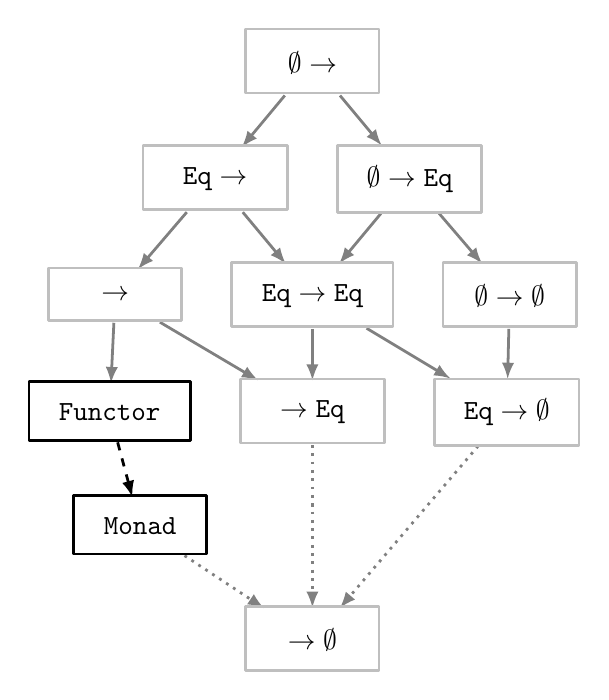
\begin{tikzpicture}[>=latex,line join=bevel,]
  \pgfsetlinewidth{1bp}
%%
\pgfsetcolor{black}
  % Edge: \kindStar \to \kindStar -> \kindStar \to \texttt{Eq}
  \pgfsetcolor{gray}
  \draw [->] (47.111bp,126.47bp) .. controls (54.966bp,121.82bp) and (64.649bp,116.09bp)  .. (82.411bp,105.59bp);
  % Edge: \emptyset \to \texttt{Eq} -> \emptyset \to \emptyset
  \draw [->] (147.61bp,165.63bp) .. controls (150.36bp,162.41bp) and (153.39bp,158.88bp)  .. (163.09bp,147.57bp);
  % Edge: \texttt{Eq} \to \texttt{Eq} -> \texttt{Eq} \to \emptyset
  \draw [->] (121.5bp,124.3bp) .. controls (128.1bp,120.34bp) and (135.62bp,115.83bp)  .. (151.63bp,106.22bp);
  % Edge: \emptyset \to \texttt{Eq} -> \texttt{Eq} \to \texttt{Eq}
  \draw [->] (126.69bp,165.63bp) .. controls (124.01bp,162.41bp) and (121.06bp,158.88bp)  .. (111.64bp,147.57bp);
  % Edge: \emptyset \to \kindStar -> \emptyset \to \texttt{Eq}
  \draw [->] (111.94bp,208.08bp) .. controls (114.57bp,204.91bp) and (117.49bp,201.41bp)  .. (126.92bp,190.1bp);
  % Edge: \texttt{Eq} \to \texttt{Eq} -> \kindStar \to \texttt{Eq}
  \draw [->] (102bp,124.08bp) .. controls (102bp,121.44bp) and (102bp,118.57bp)  .. (102bp,105.52bp);
  % Edge: \emptyset \to \kindStar -> \texttt{Eq} \to \kindStar
  \draw [->] (92.064bp,208.08bp) .. controls (89.26bp,204.71bp) and (86.135bp,200.96bp)  .. (76.599bp,189.52bp);
  % Edge: \texttt{\texttt{Monad}} -> \kindStar \to \emptyset
  \draw [->,dotted] (55.967bp,42.441bp) .. controls (62.122bp,38.371bp) and (69.321bp,33.61bp)  .. (84.562bp,23.532bp);
  % Edge: \texttt{Eq} \to \kindStar -> \texttt{Eq} \to \texttt{Eq}
  \draw [->] (76.936bp,166.08bp) .. controls (79.74bp,162.71bp) and (82.865bp,158.96bp)  .. (92.401bp,147.52bp);
  % Edge: \texttt{Eq} \to \emptyset -> \kindStar \to \emptyset
  \draw [->,dotted] (161.67bp,81.901bp) .. controls (150.38bp,68.669bp) and (132.11bp,47.267bp)  .. (111.92bp,23.618bp);
  % Edge: \texttt{Eq} \to \kindStar -> \kindStar \to \kindStar
  \draw [->] (56.78bp,166.08bp) .. controls (53.385bp,162.12bp) and (49.533bp,157.62bp)  .. (39.189bp,145.55bp);
  % Edge: \kindStar \to \kindStar -> \texttt{\texttt{Functor}}
  \draw [->] (30.536bp,126.26bp) .. controls (30.372bp,122.81bp) and (30.18bp,118.78bp)  .. (29.503bp,104.57bp);
  % Edge: \texttt{\texttt{Functor}} -> \texttt{\texttt{Monad}}
  \pgfsetcolor{black}
  \draw [->,dashed] (31.89bp,83.228bp) .. controls (32.705bp,80.191bp) and (33.619bp,76.783bp)  .. (37.167bp,63.559bp);
  % Edge: \kindStar \to \texttt{Eq} -> \kindStar \to \emptyset
  \pgfsetcolor{gray}
  \draw [->,dotted] (102bp,82.251bp) .. controls (102bp,69.708bp) and (102bp,49.542bp)  .. (102bp,23.727bp);
  % Edge: \emptyset \to \emptyset -> \texttt{Eq} \to \emptyset
  \draw [->] (172.72bp,124.08bp) .. controls (172.66bp,121.62bp) and (172.59bp,118.95bp)  .. (172.29bp,106.1bp);
  % Node: \emptyset \to \texttt{Eq}
\begin{scope}
  \definecolor{strokecol}{rgb}{0.75,0.75,0.75};
  \pgfsetstrokecolor{strokecol}
  \draw (163bp,190bp) -- (111bp,190bp) -- (111bp,166bp) -- (163bp,166bp) -- cycle;
  \definecolor{strokecol}{rgb}{0.0,0.0,0.0};
  \pgfsetstrokecolor{strokecol}
  \draw (137bp,178bp) node {$\emptyset \to \texttt{Eq}$};
\end{scope}
  % Node: \texttt{\texttt{Monad}}
\begin{scope}
  \definecolor{strokecol}{rgb}{0.0,0.0,0.0};
  \pgfsetstrokecolor{strokecol}
  \draw (64bp,64bp) -- (16bp,64bp) -- (16bp,43bp) -- (64bp,43bp) -- cycle;
  \draw (40bp,53bp) node {$\texttt{\texttt{Monad}}$};
\end{scope}
  % Node: \kindStar \to \texttt{Eq}
\begin{scope}
  \definecolor{strokecol}{rgb}{0.75,0.75,0.75};
  \pgfsetstrokecolor{strokecol}
  \draw (128bp,106bp) -- (76bp,106bp) -- (76bp,83bp) -- (128bp,83bp) -- cycle;
  \definecolor{strokecol}{rgb}{0.0,0.0,0.0};
  \pgfsetstrokecolor{strokecol}
  \draw (102bp,94bp) node {$\kindStar \to \texttt{Eq}$};
\end{scope}
  % Node: \texttt{Eq} \to \kindStar
\begin{scope}
  \definecolor{strokecol}{rgb}{0.75,0.75,0.75};
  \pgfsetstrokecolor{strokecol}
  \draw (93bp,190bp) -- (41bp,190bp) -- (41bp,167bp) -- (93bp,167bp) -- cycle;
  \definecolor{strokecol}{rgb}{0.0,0.0,0.0};
  \pgfsetstrokecolor{strokecol}
  \draw (67bp,178bp) node {$\texttt{Eq} \to \kindStar$};
\end{scope}
  % Node: \emptyset \to \kindStar
\begin{scope}
  \definecolor{strokecol}{rgb}{0.75,0.75,0.75};
  \pgfsetstrokecolor{strokecol}
  \draw (126bp,232bp) -- (78bp,232bp) -- (78bp,209bp) -- (126bp,209bp) -- cycle;
  \definecolor{strokecol}{rgb}{0.0,0.0,0.0};
  \pgfsetstrokecolor{strokecol}
  \draw (102bp,220bp) node {$\emptyset \to \kindStar$};
\end{scope}
  % Node: \kindStar \to \kindStar
\begin{scope}
  \definecolor{strokecol}{rgb}{0.75,0.75,0.75};
  \pgfsetstrokecolor{strokecol}
  \draw (55bp,146bp) -- (7bp,146bp) -- (7bp,127bp) -- (55bp,127bp) -- cycle;
  \definecolor{strokecol}{rgb}{0.0,0.0,0.0};
  \pgfsetstrokecolor{strokecol}
  \draw (31bp,136bp) node {$\kindStar \to \kindStar$};
\end{scope}
  % Node: \texttt{Eq} \to \texttt{Eq}
\begin{scope}
  \definecolor{strokecol}{rgb}{0.75,0.75,0.75};
  \pgfsetstrokecolor{strokecol}
  \draw (131bp,148bp) -- (73bp,148bp) -- (73bp,125bp) -- (131bp,125bp) -- cycle;
  \definecolor{strokecol}{rgb}{0.0,0.0,0.0};
  \pgfsetstrokecolor{strokecol}
  \draw (102bp,136bp) node {$\texttt{Eq} \to \texttt{Eq}$};
\end{scope}
  % Node: \texttt{\texttt{Functor}}
\begin{scope}
  \definecolor{strokecol}{rgb}{0.0,0.0,0.0};
  \pgfsetstrokecolor{strokecol}
  \draw (58bp,105bp) -- (0bp,105bp) -- (0bp,84bp) -- (58bp,84bp) -- cycle;
  \draw (29bp,94bp) node {$\texttt{\texttt{Functor}}$};
\end{scope}
  % Node: \kindStar \to \emptyset
\begin{scope}
  \definecolor{strokecol}{rgb}{0.75,0.75,0.75};
  \pgfsetstrokecolor{strokecol}
  \draw (126bp,24bp) -- (78bp,24bp) -- (78bp,1bp) -- (126bp,1bp) -- cycle;
  \definecolor{strokecol}{rgb}{0.0,0.0,0.0};
  \pgfsetstrokecolor{strokecol}
  \draw (102bp,12bp) node {$\kindStar \to \emptyset$};
\end{scope}
  % Node: \texttt{Eq} \to \emptyset
\begin{scope}
  \definecolor{strokecol}{rgb}{0.75,0.75,0.75};
  \pgfsetstrokecolor{strokecol}
  \draw (198bp,106bp) -- (146bp,106bp) -- (146bp,82bp) -- (198bp,82bp) -- cycle;
  \definecolor{strokecol}{rgb}{0.0,0.0,0.0};
  \pgfsetstrokecolor{strokecol}
  \draw (172bp,94bp) node {$\texttt{Eq} \to \emptyset$};
\end{scope}
  % Node: \emptyset \to \emptyset
\begin{scope}
  \definecolor{strokecol}{rgb}{0.75,0.75,0.75};
  \pgfsetstrokecolor{strokecol}
  \draw (197bp,148bp) -- (149bp,148bp) -- (149bp,125bp) -- (197bp,125bp) -- cycle;
  \definecolor{strokecol}{rgb}{0.0,0.0,0.0};
  \pgfsetstrokecolor{strokecol}
  \draw (173bp,136bp) node {$\emptyset \to \emptyset$};
\end{scope}
%
\end{tikzpicture}

